%; whizzy chapter
% -initex iniptex -latex platex -format platex -bibtex jbibtex -fmt fmt
% 以上 whizzytex を使用する場合の設定.

%     Kansai Debian Meeting resources
%     Copyright (C) 2007 Takaya Yamashita
%     Thank you for Tokyo Debian Meeting resources

%     This program is free software; you can redistribute it and/or modify
%     it under the terms of the GNU General Public License as published by
%     the Free Software Foundation; either version 2 of the License, or
%     (at your option) any later version.

%     This program is distributed in the hope that it will be useful,
%     but WITHOUT ANY WARRANTY; without even the implied warranty of
%     MERCHANTABILITY or FITNESS FOR A PARTICULAR PURPOSE.  See the
%     GNU General Public License for more details.

%     You should have received a copy of the GNU General Public License
%     along with this program; if not, write to the Free Software
%     Foundation, Inc., 51 Franklin St, Fifth Floor, Boston, MA  02110-1301 USA

%  preview (shell-command (concat "evince " (replace-regexp-in-string "tex$" "pdf"(buffer-file-name)) "&"))
% 画像ファイルを処理するためには ebb を利用して boundingbox を作成.
%(shell-command "cd image200708; ebb *.png")

%%ここからヘッダ開始.

\documentclass[mingoth,a4paper]{jsarticle}
\usepackage{kansaimonthlyreport}
\usepackage[dvips]{xy}
\usepackage{ascmac}

% 日付を定義する, 毎月変わります.
\newcommand{\debmtgyear}{2011}
\newcommand{\debmtgdate}{26}
\newcommand{\debmtgmonth}{06}
\newcommand{\debmtgnumber}{48}

\begin{document}

\begin{titlepage}

% 毎月変更する部分, 本文の末尾も修正することをわすれずに

 第\debmtgnumber{}回 関西 Debian 勉強会資料

\vspace{2cm}

\begin{center}
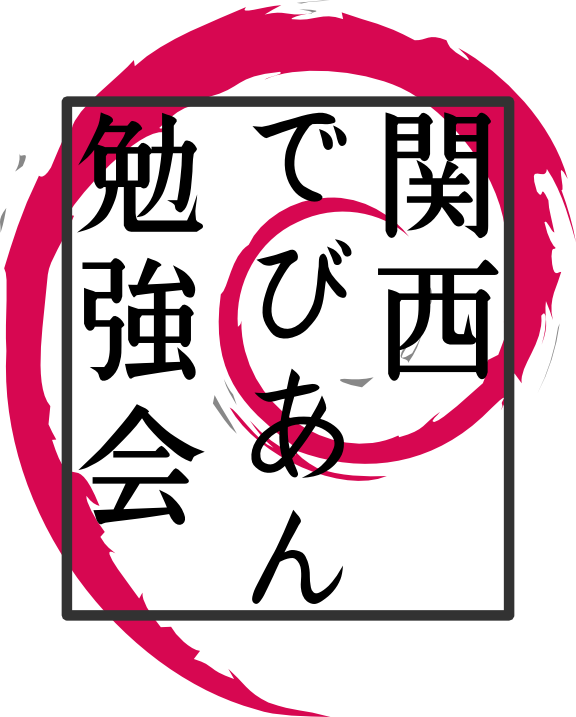
\includegraphics{image200802/kansaidebianlogo.png}
\end{center}

\begin{flushright}
\hfill{}関西 Debian 勉強会担当者 佐々木・倉敷・のがた \\
\hfill{}\debmtgyear{}年\debmtgmonth{}月\debmtgdate{}日
\end{flushright}

\thispagestyle{empty}
\end{titlepage}

\dancersection{Introduction}{Debian JP}

\subsection*{}%ロゴ用のスペース稼ぎ

関西 Debian 勉強会は Debian GNU/Linux のさまざまなトピック (新しいパッケー
ジ, Debian 特有の機能の仕組, Debian 界隈で起こった出来事, などなど) に
ついて話し合う会です.

目的として次の三つを考えています.
\begin{itemize}
      \item ML や掲示板ではなく, 直接顔を合わせる事での情報交換の促進
      \item 定期的に集まれる場所
      \item 資料の作成
\end{itemize}

それでは, 楽しい一時をお楽しみ下さい.

\clearpage

\begin{minipage}[b]{0.2\hsize}
 {\rotatebox{90}{\fontsize{80}{80}
{\gt 関西 Debian 勉強会}}}
\end{minipage}
\begin{minipage}[b]{0.8\hsize}
\hrule
\vspace{2mm}
\hrule
\setcounter{tocdepth}{1}
\tableofcontents
\vspace{2mm}
\hrule
\end{minipage}


\dancersection{最近の Debian 関係のイベント報告}{Debian JP}

\subsection{OSC 2011 Sendai 出張Debian勉強会}

2011年5月21日(土)に宮城県仙台市でオープンソースカンファレンス2011仙台が開
催されました。

Debian勉強会では吉田@板橋が展示で出展しました。
\begin{enumerate}
\item「東京エリアDebian勉強会/関西Debian勉強会」の紹介
\item「あんどきゅめんてっどでびあん(Debian勉強会資料のサマリ)」の展示、販売
\item「Debian Squeezeの展示」具体的には「Debian GNU/kFreeBSD」の展示
\end{enumerate}
主に上記をおこないました。
メインホール入り口正面という配置にも恵まれ、多くの方に立ち寄って頂きました。

\begin{center}
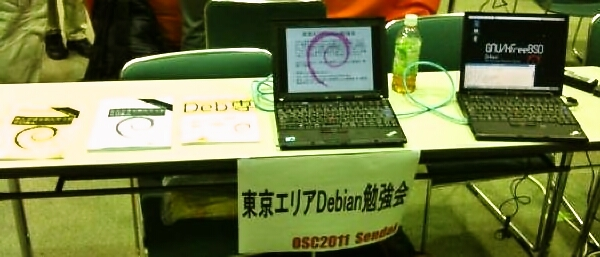
\includegraphics[width=10cm]{image201106/oscsendai.jpg}
\end{center}

また, 関西からはのがたさんが参加されています。今日時間があれば、お話を伺いたい所です。

\subsection{OSC 2011 Hokkaido 出張Debian勉強会}

2011年6月11日(土)に北海道札幌市でオープンソースカンファレンス2011北海道が開催されました。

Debian勉強会ではタイトル「Debian 6.0(squeeze) \& Debian Update」として佐々木がセッションを行いました。
セッションには14名が参加し、質問ではバグ報告の手順を確認する質問が出されました。

GPGキーサインパーティの参加者はコーディネーターを含めて3名でした。
「ある程度知識のある人々は既に必要な人とキーサインを終えているし、そうでない人はそもそも GPG に興味すらない現状をなんとかしないといけないですね」
というご意見も頂きました。GPG の啓蒙活動を引き続き行っていく必要がありそうです
\footnote{来月の OSC Kansai\@Kyotoでも GPG キーサインパーティを開催する予定です。よろしくお願いします!}。

\begin{center}
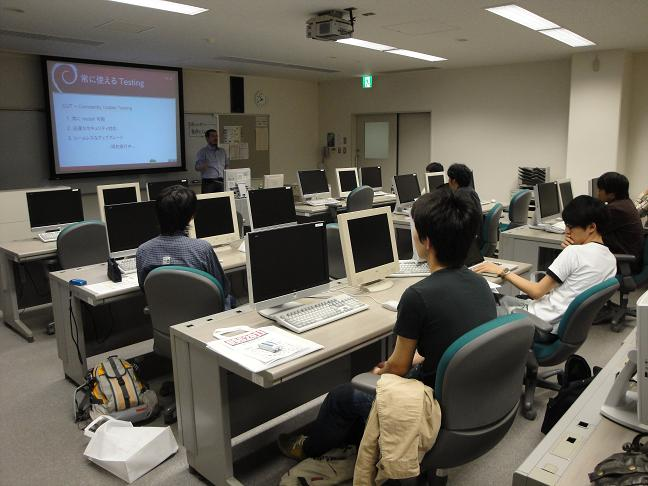
\includegraphics[width=10cm]{image201106/osc11do.jpg}
\end{center}

\subsection{第 77 回東京エリアDebian勉強会}

2011年6月18日(土)に第77回東京エリアDebian勉強会が開催されました。
上川さんによる XSLT による Debian JP 定例会議議事録処理系の話や
前田さんによる Sphnix および Doxygen の話がありました。
詳細は PDF 公開資料をご覧下さい%
\footnote{Doxygen についてはちょっと深追いしている所なので、そのうち機会があったらお話できると良いな、と思っています(佐々木)}

\subsection{Debian 6.0.2 released}

Squeeze の二つ目の point release となる Debian 6.0.2 が 2011年 6 月 25 日(この原稿を書いている最中)にリリースされました。
\begin{center}
  {\tt{http://www.debian.org/News/2011/20110625}}
\end{center}
多くの bugfix、security fix がなされています。詳細は上記 URL をご覧下さい。

\subsection{Debian JP なう}

ご存知の方もいらっしゃるかもしれませんが、twitter アカウント{\tt{debianjp}} が最近活発に活動中です。
Debian JP の中の人が呟いております。 まだフォローしていない方は是非どうぞ!

\clearpage
%-------------------------------------------------------------------------------
\dancersection{事前課題}{Debian JP}

今回は以下の事前課題を設定しました。

\begin{enumerate}
\item http://test-ipv6.jp/ で IPv6 接続性をテストしてください。(出来れば複数の環境で)
\item World IPv6 Day (以降) で何か影響がありましたか。(例: 特定のサイトへのアクセスが遅くなった、何度かリロードしないと表示されなくなった)
\item Debian パッケージを作成した事の無い人は Debian のソースパッケージの構成を復習しておいて下さい.
\end{enumerate}

参加者の皆さんによる回答は以下の通りです(一部こちらで整形してます。ご容赦
下さい)。

\begin{prework}{ 佐々木洋平 }
  直前に回答する駄目な人です。
  \begin{enumerate}
  \item 北大、京都大、神戸大、九大の学内にある計算機からテストしました
    が、v6 は軒並駄目です。 とはいえ、大学毎の情報基盤センター(に類する所)で
    トンネルなりなんなり噛ませていると思いますので、まあそういうモンかな、
    とか思ったり。
  \item 特にこれといって不具合もなく.
  \item source format 3.0 (git) とか soruce format 3.0 (bzr) いうモノの存
    在を知ってモニョっとしました。
  \end{enumerate}
\end{prework}

\begin{prework}{ 古川竜雄 (frkwtto@gmail.com) }
  \begin{enumerate}
  \item {\tt{http://test-ipv6.jp/}} で IPv6 接続性をテストしてください
\begin{commandline}
* 一般のインターネット上で見えるあなたの IPv4 アドレスは ***
* IPv6 アドレスが検出されませんでした
* World IPv6 Dayは2011年6月8日です。このブラウザ、この場所からは問題ないことが予想されます。
* あなたは IPv4 インターネットのみを閲覧できるようです。あなたは IPv6 のみのサイトに到達できません。
* あなたの DNS サーバ (おそらくお使いのプロバイダが運用) は、IPv6 インターネットアクセスがない、もしくは利用しないように設定されているようです。このため、将来的に、IPv6 のみに対応したサイトへの到達できない恐れがあります。
あなたの事前対応点
10/10  コンテンツ側が IPv4 および IPv6 を提供した際の、あなたの IPv4 の安定性と準備状況
 0/10  コンテンツ側が IPv6 のみになった際の、あなたの IPv6 の安定性と準備状況
\end{commandline}
    Yahoo BBとぷららで全く同じ結果を示しました。
\begin{commandline}
# cat /proc/version
Linux version 2.6.26-2-686 (Debian 2.6.26-26lenny1) (dannf@debian.org) \\
(gcc version 4.1.3 20080704 (prerelease)
(Debian 4.1.2-25)) #1 SMP Thu Nov 25 01:53:57 UTC 2010
\end{commandline}
  \item World IPv6 Day (以降) で何か影響がありましたか。\\
    何も変わりません。IPv6を使ってないから??
  \end{enumerate}
\end{prework}

\begin{prework}{ 水野源 }
  \begin{enumerate}
  \item 我が家はv4しか使えません!
  \item 特になし
  \end{enumerate}
\end{prework}

\begin{prework}{ やつお }
  \begin{enumerate}
  \item 3ヶ所から試してみましたが全て「×IPv6アドレス が検出されませんでした」となりました。
  \item あまり意識していないのですが、特に問題無いと思います。
  \item 勉強しておきます…
  \end{enumerate}
\end{prework}

\begin{prework}{ kaimasami0001 }
  \begin{description}
  \item[課題1] 次の(a),(b)2環境を用意しました。
    \def\theenumi{(\alph{enumi})}
    \begin{enumerate}
    \item ネイティブdebian squeeze(64bit)
    \item 上の環境上のkvm-qemu上のdebian squeeze(32bit)
    \end{enumerate}
    \def\theenumi{\arabic{enumi}}
両環境ともOS上ではIPv6の設定をしていない、私のプロバイダは今年5〜7月にIPv6に対応中、ということで、http://test-ipv6.jp/への接続結果もそれなりの結果でした。
\begin{commandline}
  10/10  コンテンツ側が IPv4 および IPv6 を提供した際の、
         あなたの IPv4 の安定性と準備状況
   0/10  コンテンツ側が IPv6 のみになった際の、あなたの
         IPv6 の安定性と準備状況
\end{commandline}
\item[課題2] World IPv6 Day (以降) での影響\\
10秒〜20秒まっても表示しないサイトがありました。それまで見たことのないサイトだったので原因がIPv6のせいかどうかは不明。
\item[課題3] Debianソースパッケージの構成の復習\\
  すみません。復習はまだです。
  \end{description}
\end{prework}

\begin{prework}{ 山田 洋平 }
  \begin{enumerate}
  \item IPv6 に対応していないけど、みんな同じだから大丈夫。みたいに言われました。(自宅からと携帯電話からと)
  \item 話には聞いていましたが何も気付きませんでした。
  \item 土曜日見ておきます。
  \end{enumerate}
\end{prework}

\begin{prework}{ 小林 克希 }
  \begin{enumerate}
  \item 自宅も会社もIPv4 10/10, IPv6 0/10でした。
  \item あまり気づいた点はないです。(そもそも、昔に比べてwebを見なくなってしまったのもあるのですが……。)
  \item 一応、Ubuntuに勝手に自前パッケージを取り込まれたことくらいはあるのですが(笑)、もう数年前の話でほとんど覚えてないので復習しておきます。
  \end{enumerate}
初参加の者です。
参加表明がギリギリとなってしまい申し訳ございません。
昨年の10月に大阪に引っ越してきました。
Debianは学生時代はよくいじっていたのですが、
最近はさっぱりでsqueezeのリリースにも全然気づいてませんでした……。
せっかくの機会ですので、また少しいじってみたいと思っています。
よろしくお願いします。
\end{prework}

\begin{prework}{ かわだてつたろう }
  \begin{enumerate}
  \item WiMAX から行ないましたが事前対応点の IPv6 は 0/10 でした。
  \item 影響を感じるようなことはありませんでした。
  \item hello のパッケージを再作成してみました。DEP-5 フォーマットで書くのはかなり大変ですね。
  \end{enumerate}
\end{prework}

\begin{prework}{ 佐藤誠 }
  \begin{enumerate}
  \item 一応アクセスはしましたが、V6を優先にできませんでした。
  \item 基本的に非対応の環境におりました。何も変わったことはないです。
  \item 確認します。
  \end{enumerate}
\end{prework}

\begin{prework}{ 松澤二郎 }
  \begin{enumerate}
  \item
\begin{commandline}
IPv4 DNS レコードのテスト
ok (0.456s) 利用 ipv4
IPv6 DNS レコードのテスト
bad (0.365s)
デュアルスタック DNS レコードのテスト
ok (0.506s) 利用 ipv4
デュアルスタック DNS と大きなパケットのテスト
ok (0.364s) 利用 ipv4
DNSを利用しないIPv4のテスト
ok (0.332s) 利用 ipv4
DNSを利用しないIPv6のテスト
bad (0.054s)
IPv6 ラージパケットのテスト
bad (0.043s)
お使いのプロバイダのDNSサーバのIPv6の利用状況のテスト
bad (0.885s)
\end{commandline}
  \item 特にありません。
  \item
    実用途ではパッケージ作成は未経験です。
    「Debian パッケージ 60 分クッキング」を見ました。
  \end{enumerate}
\end{prework}

\begin{prework}{ 木下 }
  \begin{enumerate}
  \item IPv6 接続性テスト
\begin{commandline}
IPv4 DNS レコードのテスト・・・ok (0.486s) 利用 ipv4
IPv6 DNS レコードのテスト・・・bad (0.017s)
デュアルスタック DNS レコードのテスト・・・ok (3.497s) 利用 ipv4
デュアルスタック DNS と大きなパケットのテスト・・・ok (0.078s) 利用 ipv4
DNSを利用しないIPv4のテスト・・・ok (0.482s) 利用 ipv4
DNSを利用しないIPv6のテスト・・・bad (0.004s)
IPv6 ラージパケットのテスト・・・bad (0.004s)
お使いのプロバイダのDNSサーバのIPv6の利用状況のテスト・・・ok (3.453s) 利用 ipv4
\end{commandline}
    結論:私の自宅のネット環境ではIPV6は無理かも・・・
  \item World IPv6 Day (以降) で何か影響がありましたか。\\
    今のところ、特になし。
  \end{enumerate}
\end{prework}

\begin{prework}{ lurdan }
  \begin{enumerate}
  \item IPv6 でつながる環境は所持していないようです
  \item 特にネガティブな影響もなく、完全に他人事でした。
  \item いちおう。しってる。つもり。
  \end{enumerate}
\end{prework}

\begin{prework}{ よしだともひろ }
  \begin{enumerate}
  \item {\tt{http://test-ipv6.jp/}} での接続性テスト
    (自宅で実施した際のサマリー)
\begin{commandline}
一般のインターネット上で見えるあなたの IPv4 アドレスはXXX.XXX.XXX.115
IPv6 アドレスが検出されませんでした
World IPv6 Dayは2011年6月8日です。このブラウザ、この場所からは問題ないことが予想されます。
あなたは IPv4 インターネットのみを閲覧できるようです。あなたは IPv6 のみのサイトに到達できません。
あなたの DNS サーバ (おそらくお使いのプロバイダが運用) は、IPv6 インターネットアクセスがあるように思われます。
 あなたの事前対応点
10/10  コンテンツ側が IPv4 および IPv6 を提供した際の、あなたの IPv4 の安定性と準備状況
 0/10  コンテンツ側が IPv6 のみになった際の、あなたの IPv6 の安定性と準備状況
\end{commandline}
  \item World IPv6 Day (以降) で何か影響がありましたか。 \\
    現在のところ、特に問題はないように思います。
  \item Debian のソースパッケージの構成を復習
  \item
つい最近『入門Debianパッケージ』を入手して、読み始めたところです。「古いので今から読むのはやめといた方がよい」というようなことはないでしょうか?
  \end{enumerate}
\end{prework}

\begin{prework}{ kozo2 }
  \begin{enumerate}
  \item WiMAXでこのようになりました
\begin{commandline}
IPv4 DNS レコードのテスト
ok (0.208s) 利用 ipv4
IPv6 DNS レコードのテスト
bad (0.106s)
デュアルスタック DNS レコードのテスト
ok (0.140s) 利用 ipv4
デュアルスタック DNS と大きなパケットのテスト
ok (0.207s) 利用 ipv4
DNSを利用しないIPv4のテスト
ok (0.112s) 利用 ipv4
DNSを利用しないIPv6のテスト
bad (0.013s)
IPv6 ラージパケットのテスト
bad (0.012s)
お使いのプロバイダのDNSサーバのIPv6の利用状況のテスト
bad (0.011s)
\end{commandline}
  \item 特にありませんでした
  \item 前回(第 47 回 関西 Debian 勉強会)のlurdanさんのdpkgのおさらいを見ました
  \end{enumerate}
\end{prework}

\begin{prework}{ 川江 }
  \begin{enumerate}
  \item 私の事前対応状況は以下です。
\begin{commandline}
10/10  コンテンツ側が IPv4 および IPv6 を提供した際の、あなたの IPv4 の安定性と準備状況
 0/10  コンテンツ側が IPv6 のみになった際の、あなたの IPv6 の安定性と準備状況
2.特になし。
\end{commandline}
  \end{enumerate}
\end{prework}

\begin{prework}{ 山下康成 }
  \begin{enumerate}
  \item (藁
\begin{commandline}
  10/10  コンテンツ側が IPv4 および IPv6 を提供した際の、あなたの IPv4 の安定性と準備状況
   0/10  コンテンツ側が IPv6 のみになった際の、あなたの IPv6 の安定性と準備状況
\end{commandline}
  \item 何も気がつきませんでした
  \item Debian パッケージ 60分クッキングをざっと見ました。
    必要な技能は備わっているようです。
    sh script は読み書きできます。
    Makefile もまぁまぁ読み書きできます。
    好奇心は、、、、
  \end{enumerate}
\end{prework}

\clearpage
%------------------------------------------------------------------------------
\dancersection{IPv6 のトンネル接続を試してみた話}{西山和広}
\subsection{概要}

今回の話は、プロバイダが IPv6 ネイティブ接続にまだ対応していない状況、つまり
直接外に繋がるのは IPv4 のみの接続の環境で IPv6 を使う話です。
\subsection{IPv6 概要}

\subsubsection{IPv6 とは何か}


最近は情報が増えてきているので省略します。
古い情報だと RFC が更新されていたり廃止されていたりして、
現状とは合わなくなっているものもあるので注意が必要です。
\subsubsection{IPv6 の利点と欠点}

IPv6 の利点としては以下のようなものが思いつきます。

\begin{itemize}
\item アドレス空間が広い
\item 実装が普及している
\item 機能的な利点はそんなにない

\begin{itemize}
\item IPsec とか Mobile IP とか IPv4 でも可能
\end{itemize}

\end{itemize}


IPv6 の欠点としては以下のようなものが思いつきます。

\begin{itemize}
\item IPv4 と互換性がない
\item まだ広く利用されていない

\begin{itemize}
\item トラブルの対処方法とかあまりない
\end{itemize}

\end{itemize}
\subsubsection{なぜ IPv6 を試そうと思ったか}

試し始めてから World IPv6 Day が実施されるなど、状況がどんどん変わっていますが、
試そうと思った最初の理由は以下のようなものです。

\begin{itemize}
\item JPNIC の IPv4 アドレスも枯渇したから
\item おもしろそうだったから
\item 余裕のあるうちにのんびりとやりたかったから

\begin{itemize}
\item 必要になってからあわててやりたくない
\end{itemize}

\end{itemize}
\subsubsection{IPv6 対応とは}

IPv6 対応にはいろいろな状態があると思いますが、今回は以下の種類を考えてみました。

\begin{itemize}
\item クライアント側

\begin{itemize}
\item IPv6 のみのサーバに接続できる ( \url{http://ipv6.google.com/} など)
\item IPv4 と IPv6 両対応のサーバに IPv6 で接続できる (\url{http://www.kame.net/} など)
\item DNS を IPv6 経由で解決できる (/etc/resolv.conf で nameserver に IPv6 アドレスを設定)

\begin{itemize}
\item これが出来ないと IPv6 のみに移行できない
\end{itemize}

\end{itemize}

\item サーバ側

\begin{itemize}
\item IPv6 アドレス指定で接続できる (グローバル IPv6 アドレス設定)
\item ホスト名で指定した場合でも IPv6 で接続できる (DNS に AAAA レコード設定)
\end{itemize}

\end{itemize}
\subsubsection{IPv6 アドレスの表記}

IPv6 アドレスは 128 ビットを 16 ビットごとに「:」で区切って 16 進数で表記します。
省略表記が RFC 4291 で決まっていますが、省略の仕方で複数の省略表記が可能なので、
RFC 5952 で推奨表記が決められました。

\begin{itemize}
\item 例: 2001:0db8:0000:0000:0000:0000:0000:0001
\item RFC 4291, RFC 5952 のルールで省略表記

\begin{description}
\item[先頭の 0 を省略] 2001:db8:0:0:0:0:0:1
\item[0 の連続は 1 回だけ \texttt{::} で省略] 2001:db8::1
\end{description}

\item 他にはアルファベットは小文字推奨など
\item IPv4 のネットワークアドレスやサブネットマスクに相当するものは
  \texttt{2001:db8::/32} の \texttt{/32} のように
  ネットワークプレフィックスとそのビット長を付けて表記します。
\end{itemize}


\texttt{2001:db8::/32} は例示用 IPv6 アドレス (RFC 3849) になっているなど、
用途により IP アドレスの範囲が決まっています。(RFC 5156)
\subsection{トンネル}
\subsubsection{トンネルの種類}

今回試したものは

\begin{itemize}
\item teredo (RFC 4380)
\item 6to4 (RFC 3056)
\item 6rd (RFC 5969)
\end{itemize}


の 3 種類です。
ISATAP (RFC 5214) など他の方式もありますが、今回の話の対象外です。
\subsection{teredo}

\subsubsection{teredo の特徴}


teredo は以下の特徴があります。

\begin{itemize}
\item NAT の中でも使えるトンネル
\item UDP/IPv4 にカプセル化して通信
\item クライアントで使うには手軽で簡単
\item サーバには向かない (仕組みを考えるとたぶん無理)
\end{itemize}


この特徴により NAT の中から IPv6 接続したい人には便利なのですが、
外部との接続を制限すべき環境では、 firewall などで UDP の
3544 番ポートへの接続を制限する必要があります。
\subsubsection{IPv6 アドレス}


\begin{itemize}
\item 接続先でも 2001:0000::/16 のアドレス (省略しない場合 2001:0000: で
  始まる文字列の IPv6 アドレス) は teredo とわかるので WWWW:WWWW の
  部分を逆引きするなどの対処が可能です。
\item 2001:0000:XXXX:XXXX:YYYY:ZZZZ:WWWW:WWWW の形式

\begin{itemize}
\item XXXX:XXXX は Teredo サーバの IPv4 アドレスを 16 進数にしたもの
\item YYYY は NAT の種類などのフラグ
\item ZZZZ はクライアントの外部 UDP ポート番号を変換したもの
\item WWWW:WWWW は Teredo クライアントの外部 IPv4 アドレスを変換したもの
\end{itemize}

\end{itemize}
\subsubsection{使い方}


\begin{itemize}
\item Windows は XP 以降で対応しています。
\item Debian では miredo パッケージをインストールするだけで teredo で接続できます。

\begin{itemize}
\item 自動で起動
\item /etc/miredo.conf で設定
\item デフォルトの ServerAddress の teredo-debian.remlab.net はフランス
    なので、アメリカにある teredo.ipv6.microsoft.com に変更した方が
    良いかもしれません
\end{itemize}

\end{itemize}
\subsubsection{接続確認}

/sbin/ifconfig で teredo の存在を確認します。

\begin{commandline}
$ /sbin/ifconfig teredo
teredo    Link encap:不明なネット  ハードウェアアドレス 00-00-00-00-00-00-00-00-00-00-00-00-00-00-00-00
          inet6アドレス: fe80::ffff:ffff:ffff/64 範囲:リンク
          inet6アドレス: 2001:0:4137:9e76:34c1:f58:XXXX:XXXX/32 範囲:グローバル
          UP POINTOPOINT RUNNING NOARP MULTICAST  MTU:1280  メトリック:1
          RXパケット:0 エラー:0 損失:0 オーバラン:0 フレーム:0
          TXパケット:3 エラー:0 損失:0 オーバラン:0 キャリア:0
      衝突(Collisions):0 TXキュー長:500
          RXバイト:0 (0.0 B)  TXバイト:144 (144.0 B)
$
\end{commandline}

接続に成功しているとき、ログ (/var/log/syslog) に以下のように出ます。

\begin{commandline}
miredo[4105]: Starting...
miredo[4107]: New Teredo address/MTU
miredo[4107]: Teredo pseudo-tunnel started
miredo[4107]:  (address: 2001:0:4137:9e76:34c1:f58:XXXX:XXXX, MTU: 1280)
\end{commandline}
\subsection{6to4}

\subsubsection{6to4 の特徴}


6to4 はグローバル IPv4 アドレスが必要ですが、申し込みなどをしなくても誰でも自由に使えます。

トンネルの方法として、プロトコル 41 (TCP や UDP ではない) でカプセル化して IPv4 で通信します。
(他の主なプロトコルの番号は ICMP: 1, TCP: 6, UDP: 17 でその層のプロトコルを使用しています。)

anycast で自動的に近いリレールータを経由 (192.88.99.1) します。
\subsubsection{6to4 の問題点}

6to4 には以下のような問題点があるため、廃止が検討されています。

\begin{itemize}
\item 往復の経路は基本的に異なる
\item 通信経路が把握できないし制御もできない
\item トラブルがおきると対処が困難
\end{itemize}
\subsubsection{IPv6 アドレス}

接続先でも 2002::/16 のアドレス (2002: で始まる文字列の IPv6 アドレス) は
6to4 とわかるので、アクセスログ解析などでは xxx.yyy.zzz.www
を逆引きするなどの対処が可能です。

\begin{description}
\item 2002:XXYY:ZZWW::/48 が使用可能

\begin{itemize}
\item XXYYZZWW は IPv4 アドレスの xxx.yyy.zzz.www を 16 進数にしたもの
\end{itemize}

\item 2002:XXYY:ZZWW:VVVV::/64 を LAN に割り当てるなどの使い方が可能
  (VVVV は任意の値)
\end{description}
\subsubsection{使い方}

基本的には「/etc/network/interfaces」で設定するだけで使えます。

6to4によるIPv6接続(Linux編) $\ll$ さくらインターネット研究所
\url{http://research.sakura.ad.jp/2010/12/27/tunnel-6to4-linux/}
などを参考にして設定します。

以下は会社のマシンで設定したときの例です。

まず 6to4 のアドレスを計算します。

\begin{commandline}
$ printf "2002:%02x%02x:%02x%02x::1\n" 220 218 54 201
2002:dcda:36c9::1
\end{commandline}

次に tun6to4 という iface の設定を追加します。

\begin{commandline}
$ sudoedit /etc/network/interfaces
auto tun6to4
iface tun6to4 inet6 v4tunnel
address 2002:dcda:36c9::1
netmask 16
gateway ::192.88.99.1
local 220.218.54.201
endpoint any
ttl 64
\end{commandline}

最後に「sudo ifup tun6to4」で有効にします。
「auto tun6to4」も設定しているので、再起動でも有効になるはずです。
\subsubsection{接続確認}

/sbin/ifconfig で tun6to4 を確認します。

\begin{commandline}
$ /sbin/ifconfig tun6to4
tun6to4   Link encap:IPv6-in-IPv4
          inet6アドレス: 2002:dcda:36c9::1/16 範囲:グローバル
          inet6アドレス: ::220.218.54.201/128 範囲:Compat
          UP RUNNING NOARP  MTU:1480  メトリック:1
          RXパケット:55939508 エラー:0 損失:0 オーバラン:0 フレーム:0
          TXパケット:84141144 エラー:1175 損失:0 オーバラン:0 キャリア:886
      衝突(Collisions):0 TXキュー長:0
          RXバイト:5470501110 (5.0 GiB)  TXバイト:88417369465 (82.3 GiB)

$
\end{commandline}
\subsection{6rd}

\subsubsection{6rd の特徴}


\begin{itemize}
\item 6to4 と同様にリレールータを経由
\item リレールータはプロバイダが用意
\item プレフィックスもプロバイダのものになる
\item teredo や 6to4 と違って IPv4 の方が優先されるということがない
\end{itemize}
\subsubsection{使い方}


squeeze のカーネル 2.6.32 は 6rd に対応していないバージョンなので、
バックポートカーネルをインストールします。
backports の apt-line を適切に設定した後、
「sudo aptitude install -t squeeze-backports linux-image-2.6.38-bpo.2-amd64」
でインストールします。
依存関係で linux-base も更新されるようです。

6rdによるIPv6接続(概要編) $\ll$ さくらインターネット研究所
\url{http://research.sakura.ad.jp/2011/01/05/tunnel-6rd-intro/}
を参考にして「/etc/network/interfaces」に設定します。

以下はさくらの VPS で squeeze にしているマシンで設定した例です。

まず 6rd のアドレスを計算します。

\begin{commandline}
$ printf "2001:55c:%02x%02x:%02x%02x::1\n" 49 212 40 201
2001:55c:31d4:28c9::1
$
\end{commandline}

次に tun6rd という iface の設定を追加します。

\begin{commandline}
$ sudoedit /etc/network/interfaces
auto tun6rd
iface tun6rd inet6 v4tunnel
  address 2001:e41:31d4:28c9::1
  netmask 32
  local 49.212.40.201
  endpoint any
  gateway ::61.211.224.125
  ttl 64
  up ip tunnel 6rd dev tun6rd 6rd-prefix 2001:e41::/32
  up ip link set mtu 1280 dev tun6rd
\end{commandline}

最後に「sudo ifup tun6rd」で有効にします。
「auto tun6rd」も設定しているので、再起動でも有効になるはずです。
\subsubsection{接続確認}

/sbin/ifconfig で tun6rd を確認します。

\begin{commandline}
$ /sbin/ifconfig tun6rd
tun6rd    Link encap:IPv6-in-IPv4
          inet6 addr: 2001:e41:31d4:28c9::1/32 Scope:Global
          inet6 addr: ::49.212.40.201/128 Scope:Compat
          UP RUNNING NOARP  MTU:1280  Metric:1
          RX packets:16336 errors:0 dropped:0 overruns:0 frame:0
          TX packets:21361 errors:0 dropped:0 overruns:0 carrier:0
          collisions:0 txqueuelen:0
          RX bytes:1854845 (1.7 MiB)  TX bytes:6845907 (6.5 MiB)

$
\end{commandline}
\subsection{6to4 ルータ}

\subsubsection{IPv6 ルータとは}


\begin{itemize}
\item ネットワークプレフィックスや有効期限を広告 (RA (Router Advertisement): ルータ広告)
\item RA を受け取った端末が IPv6 アドレスを生成して自動設定 (RFC 4862)
\item RA によるステートレスアドレス自動設定 (SLAAC)

\begin{itemize}
\item 端末がネットワークに繋がると RS (Router Solicitation: ルータ要請) を
    「ff02::2」(全ルータアドレスあてのマルチキャスト) に送信
\item ルータが RA を「ff02::1」(全ノードアドレスあてのマルチキャスト) に送信
\item RA のプレフィックスを使って IPv6 アドレス生成
\item 重複アドレス検出 (DAD) して問題なければ利用開始
\end{itemize}

\item IPv4 の DHCP と違って RA の送信元をデフォルトルートとして自動設定
\item DNS 設定配布は別途考える必要あり

\begin{itemize}
\item DNS の設定は今のところ別途 DHCPv6 を使うのが無難?
\item RA の RDNSS というオプション (RFC 6106) は使われていない?
\end{itemize}

\end{itemize}


DNS 設定についてはすぐにはわからなかったので、
今回は IPv4 の DNS をそのまま使うことにして、
IPv6 の DNS サーバ設定はしませんでした。

セキュリティ問題も関係しているので、このあたりの仕様は
まだ更新される可能性が高いです。
\subsubsection{LAN 側 IPv6 アドレス設定}

まず LAN 側に設定するネットワークプレフィックスを決めます。

今回は 6to4 により \texttt{2002:dcda:36c9::/48} が自由に使えます。
その中から JPNIC の枯渇の日の 4 月 15 日を埋め込んで
\texttt{2002:dcda:36c9:415::/64} を使うことにしました。

ルータ広告を送信する iface には固定の IPv6 アドレスが必須のようなので、
今回はわかりやすいように先頭の \texttt{2002:dcda:36c9:415::1} を設定しました。

ネットワーク設定全体としては以下のようにしました。

\begin{commandline}
$ cat /etc/network/interfaces
auto lo
iface lo inet loopback

allow-hotplug eth0
iface eth0 inet static
address 192.168.0.2
netmask 255.255.255.0
iface eth0 inet6 static
address 2002:dcda:36c9:415::1
netmask 64

allow-hotplug eth1
iface eth1 inet static
address 220.218.54.201
netmask 255.255.255.240
gateway 220.218.54.193

auto tun6to4
iface tun6to4 inet6 v4tunnel
address 2002:dcda:36c9::1
netmask 16
gateway ::192.88.99.1
local 220.218.54.201
endpoint any
ttl 64
$
\end{commandline}
\subsubsection{radvd}

radvd は RA (ルータ広告) を送信するデーモンです。

インストールしただけでは自動起動しないので、
\texttt{/usr/share/doc/radvd/README.Debian} を参考にして設定して
起動します。

\begin{commandline}
$ sudo /etc/init.d/radvd start
Starting radvd:
* /etc/radvd.conf does not exist or is empty.
* See /usr/share/doc/radvd/README.Debian
* radvd will *not* be started.
$
\end{commandline}

まず README.Debian などを参考にして/etc/sysctl.d/ipv6.conf を作成しました。
再起動前に反映させるには「sudo sysctl -p /etc/sysctl.d/ipv6.conf」です。

\begin{commandline}
$ cat /etc/sysctl.d/ipv6.conf
net.ipv6.conf.all.accept_ra=0
net.ipv6.conf.all.forwarding=1
\end{commandline}

/etc/radvd.conf は/usr/share/doc/radvd/examples/radvd.conf.exampleを参考にして以下のように設定しました。

グローバル IP アドレスから一意に決まるものをわざわざ書くのは嫌だったので、
prefix の先頭は「0:0:0」にして「Base6to4Interface eth1;」で自動設定するようにしています。

\begin{commandline}
$ cat /etc/radvd.conf
interface eth0
{
        AdvSendAdvert on;
        MinRtrAdvInterval 3;
        MaxRtrAdvInterval 10;
        AdvDefaultPreference low;
        AdvHomeAgentFlag off;
        prefix 0:0:0:0415::/64
        {
                AdvOnLink on;
                AdvAutonomous on;
                AdvRouterAddr off;
                Base6to4Interface eth1;
                AdvPreferredLifetime 120;
                AdvValidLifetime 300;
        };
};
\end{commandline}

後は「sudo /etc/init.d/radvd start」してLAN 内のマシンにグローバル IPv6 アドレスが
割り振られることを確認したり \url{http://ipv6.google.com/} が表示できることを確認したりします。
\subsubsection{libvirt に IPv6 設定}

この libvirt の設定だけ Debian squeeze ではなく Ubuntu 11.04 (natty) で確認しています。

「virsh net-edit default」で network 要素直下に「$<$ip family='ipv6'
address='2002:dcda:36c9:415::1' prefix='64' /$>$」のように設定を追加しま
す。普通は「$<$/network$>$」の行の直前に追加すれば良いと思います。

試した環境では一度保存すると以下のように2行になってしまいましたが、XML
的にはほぼ同じなので気にしなくても良いと思います。

\begin{commandline}
<ip family='ipv6' address='2002:dcda:36c9:415::1' prefix='64'>
</ip>
\end{commandline}

全体的な例は \url{http://libvirt.org/formatnetwork.html} を参考にしてください。

これだけで自動的に virbr0 に「2002:dcda:36c9:415::1/64」のアドレスが振られたり radvd が起動したりします。
\subsection{プライバシ拡張アドレス}

RA によるステートレスアドレス自動設定 (SLAAC) で
現状の Linux の実装などでは MAC アドレスを元にした
アドレスになります。
(MAC アドレスを 1 ビット変更して FF FE を真ん中に入れる)

そのため、接続する IPv6 ネットワークが変わって
prefix が違っても接続元マシンが特定できる可能性が
あります。

その対策として、プライバシ拡張アドレス (RFC 3041) の機能を
有効にすればランダムな値から IPv6 アドレスが生成される
ようになります。

実際の設定については試していないので紹介しておくだけにします。

\begin{itemize}
\item Ubuntu Linuxで匿名アドレス(RFC3041)を有効にする \url{http://dr.slump.jp/IPv6/rfc3041/}

\begin{itemize}
\item 例: \texttt{sysctl -w net.ipv6.conf.eth0.use\_tempaddr=2}
\end{itemize}
\item 高木浩光@自宅の日記 - MacユーザはIPv6を切るか \texttt{net.inet6.ip6.use\_tempaddr=1} の設定を \\
  \url{http://takagi-hiromitsu.jp/diary/20080730.html}
\item iPhone、RFC3041 (IPv6 プライバシ拡張) に対応\\
  Kenichi Maehashi's Blog \url{http://blog.kenichimaehashi.com/?article=13044202150}
\begin{itemize}
\item iOS 4.3 のセキュリティコンテンツについて\\
  \url{http://support.apple.com/kb/HT4564?viewlocale=ja_JP&locale=ja_JP}
\end{itemize}

\end{itemize}
\subsection{firewall}

\subsubsection{注意点}


IPv6 ではルータではない一般のノードでも
ユニキャストアドレスやループバックアドレス以外に、
リンクローカルアドレスやマルチキャストアドレスなど
複数の IPv6 アドレスを持つので、
firewall の設定に IPv4 より注意が必要です。

IPv4 で OP25B などの設定をしている場合は
teredo などが抜け穴にならないように注意が必要です。
\subsection{ip6tables-apply}

\begin{itemize}
\item iptables パッケージに入っている ip6tables-restore をリモートからでも
  安全に実行できるようにするものです。
\item タイムアウトするまでに y を入力しなかったら元のルールに戻してくれるので、
  設定をミスして ssh の接続が遮断されるルールにしようとしてしまっても安全です。
\item /usr/sbin/iptables-apply で /etc/network/iptables を適用できるのと
  同様に /usr/sbin/ip6tables-apply で /etc/network/ip6tables を
  適用できます。
\item 起動時にも適用するには「/sbin/ip6tables-restore $<$ /etc/network/ip6tables」
  をどこかで実行する必要があります。
\item たとえば以下のように lo の pre-up で実行します。
\end{itemize}


\begin{commandline}
iface lo inet loopback
 pre-up /sbin/iptables-restore < /etc/network/iptables
 pre-up /sbin/ip6tables-restore < /etc/network/ip6tables
\end{commandline}
\subsection{ufw}

\begin{itemize}
\item Uncomplicated FireWall の略

\begin{itemize}
\item Ubuntu FireWall ではない
\end{itemize}

\item sudo ufw allow OpenSSH や sudo ufw allow 80/tcp などのように
  簡単に使える iptables のラッパー
\end{itemize}
\subsubsection{ufw の設定ファイル}

/etc/default/ufw で基本的な設定をして、
ufw コマンドでその他の設定をして、
before\{,6\}.rules で特殊な設定をするということに
なります。

\begin{itemize}
\item /etc/default/ufw

\begin{itemize}
\item デフォルトのポリシーなどを設定
\end{itemize}

\item /etc/ufw/ufw.conf

\begin{itemize}
\item 「ufw enable」や「ufw disable」などの設定が保存されている
\end{itemize}

\item /lib/ufw/user\{,6\}.rules

\begin{itemize}
\item ufw allow などでの設定を保存
\item なぜか /lib 以下にある
\end{itemize}

\item /etc/ufw/before\{,6\}.rules

\begin{itemize}
\item 必要なら編集
\item ポートフォワーディングなどの nat テーブルの設定は
    ufw コマンドでは出来ないので、このファイルで設定
\end{itemize}

\end{itemize}
\subsubsection{/etc/default/ufw}

\begin{itemize}
\item IPV6=yes で IPv6 も有効にする
\item IPV6=yes にする前に設定した ufw allow は IPv4 のみのまま
\item IPv6 でも許可するには sudo ufw allow 22/tcp などを実行し直す
\item from や to で IPv4 アドレスや IPv6 アドレスを指定すれば個別の設定も
  可能 (例: ufw allow in on virbr0 proto udp from 0.0.0.0/0 port 68 to
  0.0.0.0/0 port 67)
\end{itemize}


こまめに「sudo ufw status」で確認するとわかりやすいです。
IPv6 でも許可できていれば以下のように (v6) の行があります。

たとえば IPV6=no のときに「sudo ufw allow OpenSSH」で許可していて、
IPV6=yes にしてから IPv6 でも許可した場合は以下のようになります。

\begin{commandline}
$ sudo ufw status
Status: active

To                         Action      From
--                         ------      ----
OpenSSH                    ALLOW       Anywhere

$ sudo ufw allow OpenSSH
Skipping adding existing rule
Rule added (v6)
$ sudo ufw status
Status: active

To                         Action      From
--                         ------      ----
OpenSSH                    ALLOW       Anywhere
OpenSSH (v6)               ALLOW       Anywhere (v6)

$
\end{commandline}
\subsubsection{/etc/ufw/before\{,6\}.rules}

/etc/default/ufw で DEFAULT$_{\mathrm{OUTPUT}}$$_{\mathrm{POLICY}}$ を REJECT にした場合は
ufw\{,6\}-before-input と同様の icmp などの許可を
ufw\{,6\}-before-output にする必要がありました。

before.rules の ICMP の設定として

\begin{commandline}
# ok icmp codes
-A ufw-before-input -p icmp --icmp-type destination-unreachable -j ACCEPT
-A ufw-before-input -p icmp --icmp-type source-quench -j ACCEPT
-A ufw-before-input -p icmp --icmp-type time-exceeded -j ACCEPT
-A ufw-before-input -p icmp --icmp-type parameter-problem -j ACCEPT
-A ufw-before-input -p icmp --icmp-type echo-request -j ACCEPT
\end{commandline}

の下に

\begin{commandline}
-A ufw-before-output -p icmp --icmp-type destination-unreachable -j ACCEPT
-A ufw-before-output -p icmp --icmp-type source-quench -j ACCEPT
-A ufw-before-output -p icmp --icmp-type time-exceeded -j ACCEPT
-A ufw-before-output -p icmp --icmp-type parameter-problem -j ACCEPT
-A ufw-before-output -p icmp --icmp-type echo-request -j ACCEPT
\end{commandline}

を追加しました。

before6.rules の ICMPv6 の設定として

\begin{commandline}
# for stateless autoconfiguration (restrict NDP messages to hop limit of 255)
-A ufw6-before-input -p icmpv6 --icmpv6-type neighbor-solicitation -m hl --hl-eq 255 -j ACCEPT
-A ufw6-before-input -p icmpv6 --icmpv6-type neighbor-advertisement -m hl --hl-eq 255 -j ACCEPT
-A ufw6-before-input -p icmpv6 --icmpv6-type router-solicitation -m hl --hl-eq 255 -j ACCEPT
-A ufw6-before-input -p icmpv6 --icmpv6-type router-advertisement -m hl --hl-eq 255 -j ACCEPT
\end{commandline}

\begin{commandline}
# ok icmp codes
-A ufw6-before-input -p icmpv6 --icmpv6-type destination-unreachable -j ACCEPT
-A ufw6-before-input -p icmpv6 --icmpv6-type packet-too-big -j ACCEPT
-A ufw6-before-input -p icmpv6 --icmpv6-type time-exceeded -j ACCEPT
-A ufw6-before-input -p icmpv6 --icmpv6-type parameter-problem -j ACCEPT
-A ufw6-before-input -p icmpv6 --icmpv6-type echo-request -j ACCEPT
\end{commandline}

の下にそれぞれ

\begin{commandline}
-A ufw6-before-output -p icmpv6 --icmpv6-type neighbor-solicitation -m hl --hl-eq 255 -j ACCEPT
-A ufw6-before-output -p icmpv6 --icmpv6-type neighbor-advertisement -m hl --hl-eq 255 -j ACCEPT
-A ufw6-before-output -p icmpv6 --icmpv6-type router-solicitation -m hl --hl-eq 255 -j ACCEPT
-A ufw6-before-output -p icmpv6 --icmpv6-type router-advertisement -m hl --hl-eq 255 -j ACCEPT
\end{commandline}

\begin{commandline}
-A ufw6-before-output -p icmpv6 --icmpv6-type destination-unreachable -j ACCEPT
-A ufw6-before-output -p icmpv6 --icmpv6-type packet-too-big -j ACCEPT
-A ufw6-before-output -p icmpv6 --icmpv6-type time-exceeded -j ACCEPT
-A ufw6-before-output -p icmpv6 --icmpv6-type parameter-problem -j ACCEPT
-A ufw6-before-output -p icmpv6 --icmpv6-type echo-request -j ACCEPT
\end{commandline}

を追加しました。


MULTICAST は 5353/udp のみ許可の設定になっていますが、
何か問題があれば変更します。

before.rules の MULTICAST 設定変更例としては

\begin{commandline}
# allow MULTICAST mDNS for service discovery (be sure the MULTICAST line above
# is uncommented)
-A ufw-before-input -p udp -d 224.0.0.251 --dport 5353 -j ACCEPT
\end{commandline}

となっているのを以下に変更します。

\begin{commandline}
# allow MULTICAST, be sure the MULTICAST line above is uncommented
-A ufw-before-input -s 224.0.0.0/4 -j ACCEPT
-A ufw-before-output -d 224.0.0.0/4 -j ACCEPT
\end{commandline}

上記のように ICMPv6 は許可しているので、
before6.rules の変更は通常は必要ないと思います。
\subsection{tcp wrapper の設定例}

localhost と libvirt のデフォルトの LAN と
今回設定した 6to4 経由の接続のみ許可する場合は
以下のようになります。

\begin{itemize}
\item /etc/hosts.deny で「ALL: ALL」と設定
\item /etc/hosts.allow で以下のように設定
\end{itemize}


\begin{commandline}
sshd: 127.0.0.1 [::1]
sshd: 192.168.122.0/24
sshd: [2002:dcda:36c9:415::]/64
\end{commandline}
\subsection{サーバ}
\subsubsection{サーバ一般}

\texttt{netstat -lnt} で確認して tcp6 でも LISTEN していれば IPv6 対応しています。

\begin{commandline}
$ netstat -lnt | grep ':22 '
tcp        0      0 0.0.0.0:22              0.0.0.0:*               LISTEN
tcp6       0      0 :::22                   :::*                    LISTEN
$
\end{commandline}
\subsubsection{OpenSSH}

\begin{itemize}
\item 少なくとも以下の設定が IPv6 対応に影響します。

\begin{itemize}
\item /etc/ssh/sshd$_{\mathrm{config}}$

\begin{itemize}
\item ListenAddress
\item AllowUsers user@ipaddr の ipaddr 部分
\end{itemize}

\item tcp wrapper
\item ip6tables
\end{itemize}

\end{itemize}
\subsubsection{Apache2}

一部の VirtualHost を IPv6 対応環境に移動しましたが、
IP アドレスに依存する設定をしていなかったので、何も問題はありませんでした。
\subsubsection{munin}

munin が使っているライブラリが IPv6 に対応していないという理由で
munin も IPv6 に対応していませんでした。
\subsection{トラブルシューティング}
\subsubsection{ping6 で最初のパケットだけ時間がかかる}

\begin{itemize}
\item トンネル接続の場合はそういうもの
\end{itemize}
\subsubsection{ping6 でパケットロスが多い}

libvirt で libvirt で自動起動される radvd とは別に
自分で radvd を起動してしまうとping6 での確認のときに
packet loss が 70\% 以上になるなどわかりにくいトラブルになりました。

そのときに「radvd[\ldots{}]: our AdvValidLifetime on eth0 for \ldots{} doesn't
agree with \ldots{}」のようなログが出ていて、調べると
\url{http://www.wiggy.net/texts/ipv6-howto/} に radvd のようなルータ広告 (RA)
するデーモンが複数動いている場合におきる問題だということがわかったので、
libvirt で自動起動されているradvd が存在するのを確認し、手動で起動して
いた方の radvd を止めることで解決しました。
\subsubsection{ifconfig で teredo がない}

\begin{itemize}
\item miredo のログ (/var/log/syslog) で原因を調べます。
\item firewall で塞がれていないか確認します。
\item NAT の種類によっては繋らないかもしれません

\begin{itemize}
\item 以前のバージョンだと NAT の種類によっては「Unsupported symmetric
    NAT detected.」で繋らないことがありましたが、今の squeeze に入っている
    miredo 1.2.3-1 では対応しているように見えます。
\item VMware などで NAT の段数を増やすと繋がったことがあります。
\end{itemize}

\end{itemize}
\subsubsection{亀が踊らない}

\begin{itemize}
\item \url{http://www.kame.net/} で亀が踊らないときの原因の調べ方
\item IPv6 で接続可能か?

\begin{itemize}
\item \url{http://ipv6.google.com/} が表示できるか?

\begin{itemize}
\item ipv6 は AAAA のみ設定されている
\item 表示できなければ、そもそも IPv6 で外と繋っていない可能性が高い
\end{itemize}

\item 詳細は \url{http://test-ipv6.com/} や \url{http://test-ipv6.jp/} でテストする
\end{itemize}

\item getaddrinfo(3) を調べる

\begin{itemize}
\item 繋がっていれば、次に getaddrinfo(3) で IPv6 が優先されているかを調べます。
\end{itemize}

\end{itemize}
\begin{itemize}

\item getaddrinfo(3) の例: IPv6 優先\\
こういう結果が返ってくれば IPv6 で繋るはずです。

\begin{commandline}
$ getent ahosts www.kame.net
2001:200:dff:fff1:216:3eff:feb1:44d7 STREAM orange.kame.net
2001:200:dff:fff1:216:3eff:feb1:44d7 DGRAM
2001:200:dff:fff1:216:3eff:feb1:44d7 RAW
203.178.141.194 STREAM
203.178.141.194 DGRAM
203.178.141.194 RAW
\end{commandline}


\item getaddrinfo(3) の例: IPv4 のみ\\
以下のように A と AAAA が設定されているはずなのに
A レコードの情報しか返ってこない場合は、
プロバイダが ``filter-aaaa-on-v4'' の設定をしていて
フィルタされているのかもしれないので、
常用はお勧めしませんが
Google Public DNS (8.8.8.8, 8.8.4.4) を
使えば回避できるかもしれません。

\begin{commandline}
$ getent ahosts www.kame.net
203.178.141.194 STREAM orange.kame.net
203.178.141.194 DGRAM
203.178.141.194 RAW
$
\end{commandline}


\item getaddrinfo(3) の例: IPv4 優先\\
以下のような出力の場合は
teredo や 6to4 よりも IPv4 が優先されている (RFC 3484)
のが原因です。
ipv6.google.com のように IPv6 のみのサイトに接続するときだけ
teredo や 6to4 の IPv6 接続が使われるようになっています。

\begin{commandline}
$ getent ahosts www.kame.net
203.178.141.194 STREAM orange.kame.net
203.178.141.194 DGRAM
203.178.141.194 RAW
2001:200:dff:fff1:216:3eff:feb1:44d7 STREAM
2001:200:dff:fff1:216:3eff:feb1:44d7 DGRAM
2001:200:dff:fff1:216:3eff:feb1:44d7 RAW
$
\end{commandline}

RFC になっているようにこの挙動の方が望ましいので、
/etc/gai.conf で設定可能ですが、一時的に変更するだけにして
試した後は戻すべきです。

Windows は netsh でポリシーテーブルを変更すれば良いそうです\footnote{以
      下、リンクはページの都合上折り返していますが一行で}

\url{http://www.tokyo6to4.net/index.php/6to4%E3%81%AE%E5%88%A9%E7%94%A8%E6%96%B9%E6%B3%95#.E3.83.9D.E3.83.AA.E3.82.B7.E3.83.BC.E3.83.86.E3.83.BC.E3.83.96.E3.83.AB.E3.81.AE.E7.B7.A8.E9.9B.86.E6.96.B9.E6.B3.95}

\item gai.conf の設定\\
\url{http://slashdot.jp/\~ohhara/journal/519278} を参考にして
teredo で接続している場合は
/etc/gai.conf に「label 2001:0::/32   1」と設定すると
亀が踊りました。
試した後は忘れずに設定を戻しておきましょう。

RFC 3484 に関連する設定として ip addrlabel もありますが、
今回は変更しなくても大丈夫でした。

デフォルトの設定は以下のようにすべてコメントで書かれていました。

\begin{commandline}
#label ::1/128       0
#label ::/0          1
#label 2002::/16     2
#label ::/96         3
#label ::ffff:0:0/96 4
#label fec0::/10     5
#label fc00::/7      6
#label 2001:0::/32   7
\end{commandline}

teredo の場合は以下のように変更しました。

\begin{commandline}
label ::1/128       0
label ::/0          1
label 2002::/16     2
label ::/96         3
label ::ffff:0:0/96 4
label fec0::/10     5
label fc00::/7      6
label 2001:0::/32   1
\end{commandline}

6to4 で接続している場合は同様に 2002::/16 を 1 にすると亀が踊りました。

\begin{commandline}
label ::1/128       0
label ::/0          1
label 2002::/16     1
label ::/96         3
label ::ffff:0:0/96 4
label fec0::/10     5
label fc00::/7      6
label 2001:0::/32   7
\end{commandline}

glibc のリゾルバの設定ファイルになるため、
プロセスの起動時のみ読み込まれているようで、
設定の反映にはブラウザの再起動が必要でした。

glibc の設定ファイルなので静的リンクされていて
glibc を使わないバイナリなどは影響を受けないと
思います。

\end{itemize} % ends low level
\subsubsection{端末は IPv6 対応なのに IPv6 のサイトに繋がらない}

WPAD (Web Proxy Auto-Discovery Protocol) で設定していた proxy が
IPv6 対応していないサーバで動いていたために繋がらないということが
ありました。
\subsubsection{一部のサイトへのアクセスが遅い・繋がらない}

\begin{itemize}
\item IPv6 から IPv4 へのフォールバックに時間がかかっている可能性がある

\begin{itemize}
\item IPv6 経由で繋がらない原因を調べる
\item サーバ側で AAAA を登録しているのにサーバが止まっている (A の方では動いている) ということもあるらしい

\begin{itemize}
\item 根本的な対処はサーバ側でしてもらうしかない
\end{itemize}

\end{itemize}

\item Opera で何度かリロードしないと bit.ly など短縮URLの一部を展開しなくなったということがあったらしい

\begin{itemize}
\item \url{http://togetter.com/li/146832}
\item IPv6 を無効にしたら直ったという話
\end{itemize}

\end{itemize}
\subsubsection{何も変えていないのに繋がらなくなった}

\begin{itemize}
\item 上流の問題かもしれないので確認

\begin{itemize}
\item メンテナンス中ではないか

\begin{itemize}
\item 「昨日の「さくらの6rd」接続不良ですが、弊社のIPv6バックボーン側でメンテナンスが実施されていたようです。」
      \url{https://twitter.com/jq6xze\_1/status/83335591873351680}
\end{itemize}

\item radvd が止まっていないか

\begin{itemize}
\item 止まっていれば起動
\end{itemize}

\item 不正な RA が送信されていないか

\begin{itemize}
\item 不正な RA を送信しているルータを探して対処
\item Windows の ICS (インターネット接続の共有) が原因になることがあるらしい
\item 意図的に不正な RA が送信されていると対処は困難 (IPv4 の ARP spoofing に似た問題になる)
\item RFC 6105 (IPv6 Router Advertisement Guard) や RFC 3971 (SEcure Neighbor Discovery (SEND)) などで対処
\end{itemize}

\item 6to4 が廃止されてリレールータ消滅?

\begin{itemize}
\item すぐにはなさそうですが、将来的には可能性がありそうです
\end{itemize}

\item teredo サーバ停止?

\begin{itemize}
\item teredo で最初に接続する teredo サーバが停止していないか
\item teredo サーバへの接続が firewall などで止められていないか
\end{itemize}

\end{itemize}

\end{itemize}
\subsubsection{短いと通信できるのに長いと通信出来ない}

\begin{itemize}
\item MTU 問題ではないか
\end{itemize}
\subsection{まとめ}

\begin{itemize}
\item IPv6 接続はクライアントとして試すだけなら簡単でした。
\item サーバも openssh や apache2 なら問題は起きにくいようです。
\item munin や proxy など問題がなさそうと思っていたところで問題が起きることもあります。
\item IPv6 の仕様は更新され続けていて、セキュリティ問題も
  まだまだこれからのようなので、引き続き最新の情報を
  追いかけていく必要がありそうです。
\end{itemize}
\subsection{参考}

\begin{thebibliography}{0}
 \bibitem{imakaraipv6} 今からはじめるIPv6 〜プロトコル基礎編〜 \url{http://www.nic.ad.jp/ja/materials/iw/2010/proceedings/s2/iw2010-s2-01.pdf}
 \bibitem{ipv4kokatsu} 絶対わかる!IPv4枯渇対策&IPv6移行超入門 ISBN 978-4-8222-6769-8
\end{thebibliography}

%-------------------------------------------------------------------------------
\dancersection{vcs-buildpackage $\sim$git,svn編$\sim$}{佐々木 洋平}
%-------------------------------------------------------------------------------

\subsection{始めに}

今日のお題は、
パッケージ作成に Git や Subversion を使用するソフトウェアである、
{\tt{git-buildpackage}}と{\tt{svn-buildpackage}}です。
自分の抱えている野良パッケージの多くが Ruby 関連だったこともあって、
PkgRubyExtras に参加したところ、
パッケージ管理を Subversion から Git へ移行するタイミングだった様で、
(幸か不幸か)両 VCS を使用してのパッケージ作成を体験しました%
\footnote{自分一人だったら絶対 Git で作業するんですけれどね}。

そこで覚えたツールの使い方とか、実際に作業する際のハマり所とかについて簡単に紹介できたら良いな、とか思います。
とはいえ、実際にはコラボする人々(=チーム)毎に work flow があるので、あまり一般論は言えない訳ですけれど。

\subsection{バージョン管理?}

バージョン管理システム(VCS)についてはほとんど説明しませんが、簡単に。

VCS を使った事のない人に VCS の利点を説明する時、佐々木は良く「良い感じのバックアップ」という言い方をしています。
例えば
\begin{itemize}
\item 過去の変更履歴を残しておける
\item 過去の任意の状態に簡単に戻せる
\item 過去にどんな変更を行なったか、を把握しやすくする(ログをきちんと書いておく必要はありますが)
\end{itemize}

また、複数人で開発を進めている時には、同じファイルに同じ様な変更を加えている場合、
最後に保存した人の変更だけが残ってしまい(上書きされてしまい)、それ以外の変更が失なわれてしまいます。
VCS を使っていると、同じファイルへの変更は「衝突」として検出されるので、こういった事態を防ぐ事ができます。

さらに、特定のバージョンに名前をつけておき(tag と言います)そのバージョンへの変更を行なったり、新機能の開発を本番の開発と分離して進めて(本番が main line と呼ばれるのに対して、branch を分ける、branch を切る、と言います)、完成した後で本番の開発に統合したりできます。

Subversion と Git は、それぞれ「集中型VCS」と「分散型VCS」の代表です。
集中型 VCS では単一のリポジトリ(データ置き場)を開発者全員が参照し作業するのに対して、
分散型 VCS では、各人が個別にリポジトリを持ち、各々のデータを適宜同期を取って作業を進めます。
最近は分散型 VCS(DVCS と言ったりします)がトレンドですね%
\footnote{集中型VCS としては CVS なんかもありますが、今更 CVS ってのは止めた方が良いと思います。また DVCS としたは Git 以外に darcs, bzr, Mercurial なんかがあります。bzr についてはそのうち山下 尊也さんが語ってくれると思います}。

\subsection{パッケージのバージョン管理?}

さて、「パッケージのバージョン管理」って何をしているのでしょうか?
Debian パッケージを「バージョン管理」する目的は幾つかありますが、
例えば
\begin{itemize}
\item 履歴の管理。
  パッケージの変更点は debian/changelog に書かれます(書きます)が、
  実際にファイル自体を参照できると大変便利です。
\item stable に含まれたパッケージにタグを付けておく。
  \begin{itemize}
  \item セキュリティ対応などを、そのタグから派生するブランチで対応する
  \end{itemize}
\item 複数人でのパッケージメンテ/チームでのパッケージメンテ作業の環境を容易に構築できる
\item upstream が VCS を使用している場合の連携が簡単になる(かも)
\end{itemize}
...でしょうか。

\subsection{何を管理するの?}
Debian のソースパッケージは、source format 3.0 では以下のファイル群で構成されます:
\begin{description}
\item[.orig.tar.{\it{ext}}] \\
  upstream のソース。複数のソースからなる場合には基本となるソースにこの名
  前をつける。{\it{ext}}は圧縮の拡張子であ
  り、{\tt{gz}}, {\tt{bz2}}, {\tt{xz}} が使用可能。
\item[.orig-{\it{component}}.tar.{\it{ext}}]  \\
  upstream が複数のソースから構成される場合のファイル
  名。{\tt{dpkg-source -x パッケージ名.dsc}}などで展開するとファイルの中
  身は {\tt{component/}}以下の展開される。
\item[.debian.tar.{\it{ext}}] \\
  {\tt{debian/}} デイレクトリの中身
\item[.dsc] \\
  パッケージの情報。上記ファイル群のハッシュなどを記載している。
\end{description}
パッケージを VCS で管理する場合、
\begin{enumerate}
\item {\tt{.orig.tar.{\it{ext}}}}
\item {\tt{.debian.tar.{\it{ext}}}}
\end{enumerate}
のバージョンを管理することになります。

\subsection{どうするの?: svn-buildpackage 編}

では実際にどうやっているのでしょうか?
ここでは GNU Hello を例に、svn-buildpackage を使った場合について簡単に述べてみます。
なお、佐々木は既に svn-buildpackage をあまり使っていないので、
Git はまだ良くわからないけれど Subversion ならわかる、 という人向けのお話です。

\subsubsection{インストール}
\begin{commandline}
  % sudo aptitude install svn-buildpackage
\end{commandline}

\subsubsection{パッケージをリポジトリに追加する}

一度適当なパッケージを作成してみましょう。 ここでは GNU hello のパッケージが作成できたとします。
横着したい人は{\tt{apt-get source hello}}でも良いでしょう。

テストのために簡単なリポジトリを作成します。ここでは {\tt{~/Work/svn/}} 以下にリポジトリを作成します。
\begin{commandline}
  % svnadmin create ~/Work/svn/
  % svn mkdir file:///home/uwabami/Work/svn/trunk -m "create trunk"
  % svn mkdir file:///home/uwabami/Work/svn/tags -m "create tags"
  % svn mkdir file:///home/uwabami/Work/svn/branches -m "create branches"
  % svn ls file:///home/uwabami/Work/svn
  branches/
  tags/
  trunk/
\end{commandline}
次に、作成したパッケージをリポジトリに追加します。追加するコマンドは {\tt{svn-inject}} です。
\begin{commandline}
  % svn-inject -l 2 -o -c 0 hello_2.7-1.dsc file:///home/uwabami/Work/svn
\end{commandline}
svn-inject のオプションの詳細は man を見てもらうとして、ここでは
\begin{commandline}
      -l
          Layout type.
          1 (default) means package/{trunk,tags,branches,...} scheme,
          2 means the {trunk,tags,branches,...}/package scheme.
      -o
          Only keep modified files under SVN control (including the debian/ directory),
          track only parts of upstream branch

       -c number
          Checkout nothing (0), trunk directory (1) or everything (2) when
          the work is done.
\end{commandline}
を用いています. 単一のパッケージを単一のリポジトリで管理する場合には {\tt{-l 1}} が良いでしょう.

\subsubsection{パッケージのビルド}

{\tt{svn-inject}}が終わったので、リポジトリからファイルを取得してみます。
\begin{commandline}
  % svn checkout file:///home/uwabami/Work/svn/trunk svn-work
  A    trunk/hello
  A    trunk/hello/debian
  A    trunk/hello/debian/control
  A    trunk/hello/debian/source
  A    trunk/hello/debian/source/format
  ...
\end{commandline}
ここでは {\tt{svn-work}} にファイルをチェックアウトしました。
実際に {\tt{svn-work/trunk/hello}} に移動して、パッケージを作成してみます。
\begin{commandline}
  % cd svn-work/trunk/hello
  % sudo apt-get build-dep hello
  % svn-buildpackage
  Complete layout information:
          trunkDir=/home/uwabami/svn-work/trunk/hello
          trunkUrl=file:///home/uwabami/Work/svn/trunk/hello
  dpkg-checkbuilddeps
  Orig tarball not found (expected ../tarballs/hello_2.7.orig.tar.gz)
  mergeWithUpstream mode detected, looking for ../tarballs/hello_2.7.orig.tar.gz
  I: mergeWithUpstream property set, looking for upstream source tarball...
  E: Could not find the upstream source file! (should be ../tarballs/hello_2.7.orig.tar.gz)
\end{commandline}
...転びました。
{\tt{svn-buildpackage}}では、
パッケージ作成時の一時ディレクトリ({\tt{build-area}})と
upstream のソースの保管場所({\tt{tarballs}})の存在を仮定しています。
これを準備しましょう(ちなみに{\tt{svn-buildpackage}}は失敗しました時点で、これらのディレクトリが既に作成されています)。
\begin{commandline}
  % cd ..
  % ls
  build-area/  hello/  tarballs/
  % cd hello
  % uscan --download-current-version --destdir=../tarballs/
\end{commandline}
{\tt{watch}}ファイルがきちんと書かれている/書けていると、{\tt{uscan}}一発で良いので楽です。
ではもう一度パッケージをビルドしてみます。
\begin{commandline}
  % svn-buildpackage
  Complete layout information:
        buildArea=/home/uwabami/svn-work/trunk/build-area
        origDir=/home/uwabami/svn-work/trunk/tarballs
        trunkDir=/home/uwabami/svn-work/trunk/hello
        trunkUrl=file:///home/uwabami/Work/svn/trunk/hello
  ...
  dpkg-deb: `../hello_2.7-1_amd64.deb' にパッケージ `hello' を構築しています。
  signfile hello_2.7-1.dsc
  gpg: “Santiago Vila <sanvila@debian.org>”をとばします: 秘密鍵が得られません
  gpg: [stdin]: clearsign failed: 秘密鍵が得られません

  dpkg-genchanges  >../hello_2.7-1_amd64.changes
  dpkg-genchanges: including full source code in upload
  dpkg-source --after-build hello-2.7
  dpkg-buildpackage: full upload (original source is included)
  dpkg-buildpackage: warning: Failed to sign .dsc and .changes file
  Command 'dpkg-buildpackage' failed in '/home/uwabami/svn-work/trunk/build-area/hello-2.7',
  how to continue now? [Qri?]: ignore
\end{commandline}
最後の gpg sign で止まっていますので i(ignore)で終わらせましょう。どうやら上手くできたみたいですね。
あとは、通常通り debian/ 以下を更新していき、リリース時(dput/dupload時)に
タグを付けたり、branch を切ってメンテしたりしてきます。

\subsubsection{new upstream release}

upstream で新しいパッケージがリリースされた時には {\tt{svn-upgrade}} コマ
ンドを使って、新しいソースを登録します。とはいえ、今回やった様
に {\tt{debian}} ディレクトリのみを管理している場合に
は、uscan の download 先を見て、適宜更新していくだけで良いでしょう。

\subsubsection{tips?}

佐々木は以下のコマンドを alias として登録しています。
svn-pbuilder は cowbuilder 呼び出しのための wrapper スクリプトです.
\begin{commandline}
if [ -f /usr/bin/svn-buildpackage ]; then
  alias svn-b="svn-buildpackage -rfakeroot -us -uc --svn-ignore --svn-lintian --svn-dont-clean"
  alias svn-bc="svn-buildpackage --svn-builder='svn-pbuilder' --svn-lintian --svn-dont-clean"
  alias svn-bct="svn-buildpackage --svn-builder='svn-pbuilder' --svn-lintian --svn-tag --svn-retag --svn-dont-clean"
  alias svn-bcl="svn-buildpackage --svn-builder='svn-pbuilder-local' --svn-lintian --svn-dont-clean"
fi
\end{commandline}

\subsection{どうするの?: git-buildpackage 編}

以下では既存のパッケージとし
て {\tt{rabbit}}\footnote{{\tt{http://rabbit-shockers.org/}}} の更新作業
を例に、git-buildpackage を使った作業を述べてみます。

\subsubsection{インストール}

\begin{commandline}
  % sudo aptitude install git-buildpackage
\end{commandline}
Recommends に {\tt{pristine-tar}} と {\tt{cowbuilder}} があります。これらもインストールしておくと良いでしょう。
{\tt{cowbuilder}}に関しては、先月の水野さんの資料を参照して下さい。
{\tt{pristine-tar}} については後述。

\subsubsection{パッケージのリポジトリへの追加}

Git なので、リポジトリの作成とか面倒な事はありません。
既存のパッケージの Git リポジトリ作成には {\tt{git-import-dsc}} を使用します。
\begin{commandline}
  % apt-get source rabbit
  % git-import-dsc --pristine-tar rabbit_0.9.2-3.dsc
  gbp:info: No git repository found, creating one.
  Initialized empty Git repository in /home/uwabami/Downloads/rabbit/.git/
  gbp:info: Tag upstream/0.9.2 not found, importing Upstream tarball
  /usr/bin/pristine-tar: committed rabbit_0.9.2.orig.tar.gz.delta to branch pristine-tar
  gbp:info: Version '0.9.2-3' imported under 'rabbit'
\end{commandline}
この際に {\tt{--pristine-tar}} オプションをつけることを推奨します。
また、これまでのバージョンの {\tt{.dsc}} ファイルと {\tt{.orig.tar.gz}}ファイルがある場合には
{\tt{git-import-dscs}} コマンドを使うと良いでしょう。tag を良きにはからってくれます。

さて、これで{\tt{rabbit}}という Git リポジトリが作成されました。実際に中を見てみましょう。
\begin{commandline}
  % cd rabbit
  % git branch
  * master                    <-- debian/ 入りのフルソース
    pristine-tar              <-- orig.tar.{gz,bz2} のバイナリデルタ
    upstream                  <-- debian/ 無し(upstream)のソース
  % git tag
  debian/0.9.2-3
  upstream/0.9.2
\end{commandline}
ブランチの意味は上記の通りです。{\tt{git-import-dscs}} を使うと、バージョ
ンに応じて tag が沢山並んでいると思います。{\tt{master}},

{\tt{pristine-tar}}はちょっと特殊です。
このブランチには、import される前の .tar.gz(もしくは.bz2)のバイナリデルタのみがコミットされています。
{\tt{git-buildpackage}} を実行すると {\tt{upstream}}ブランチ、もしくは {\tt{upstream/バージョン番号}}タグから、
元々の {\tt{orig.tar.\{gz,bz2\}}}を生成します。
{\tt{pristine-tar}}ブランチのバイナリデルタが無いと(圧縮率が違ったりして)元々の upstream のソースを正しく生成できなかったりします。

\subsubsection{パッケージのビルド}
では、パッケージをビルドしてみましょう。
\begin{commandline}
  % sudo apt-get build-dep rabbit
  % cd rabbit
  % git-buildpackage
  ...
  ...
  Successfully signed dsc and changes files
\end{commandline}
ちなみに{\tt{notify-send}}コマンドがあると、git-buildpackage の結果を通知してくれます。

あとは通常通り{\tt{debian/}} 以下を更新していき、リリース毎にタグをつけたり、適当に branch を切って作業していきます。
また(Subversionのところでは紹介しませんでしたが) {\tt{git-dch}} コマンドによって、
Git のコミットログから {\tt{debian/changelog}} を生成することができます(コミットログの最初の行しか生かされませんので、粒度の小さいコミットが求められます)。

\subsubsection{New upstream release}

upstream で新しいリリースが出た場合には {\tt{git-import-orig}} で新しい {\tt{.orig.tar.\{gz,bz2\}}}を取り込みます。
\begin{commandline}
  % uscan --download
  rabbit: Newer version (0.9.3) available on remote site:
    http://rabbit-shockers.org/download/rabbit-0.9.3.tar.gz
    (local version is 0.9.2)
  rabbit: Successfully downloaded updated package rabbit-0.9.3.tar.gz
      and symlinked rabbit_0.9.3.orig.tar.gz to it
  % git-import-orig --pristine-tar ../rabbit_0.9.3.orig.tar.gz
  What is the upstream version? [0.9.3]
  gbp:info: Importing '../rabbit_0.9.3.orig.tar.gz' to branch 'upstream'...
  gbp:info: Source package is rabbit
  gbp:info: Upstream version is 0.9.3
  /usr/bin/pristine-tar: committed rabbit_0.9.3.orig.tar.gz.delta to branch pristine-tar
  gbp:info: Merging to 'master'
  ...
  gbp:info: Successfully imported version 0.9.3 of ../rabbit_0.9.3.orig.tar.gz
\end{commandline}
既存の master と自動的に merge が行なわれますので、適宜修正してきます。

\subsubsection{patch-queue ブランチ?}

source format 3.0 (quilt) では, upstream への変更点を {\tt{quilt}} を用い
てパッチで管理します。通常通り {\tt{quilt}} を用いてパッチを作成(もしく
は debuild が走ったさいにパッチとして抽出)するのでも良いのですが、
折角なので{\tt{git format-patch}}でパッチを生成する方法について述べてみます。

{\tt{git-buildpackage}} には {\tt{gbp-pq}}というコマンドが提供されています。pq は patch-queue の略です。
先ず、現時点で debian/patches 以下にあるパッチを {\tt{patch-queue}} ブランチへ登録します。
\begin{commandline}
  % quilt pop -a
  % gbp-pq import
\end{commandline}
この時点で、{\tt{master}} ブランチから {\tt{patch-queue/master}} ブランチへ切り代わります。
debian/patches 以下にあったパッチがファイル一つ毎に一つのコミットとして登録されます。
適宜 rebase するなどして、パッチをマージしたり削除したりしていきます。
パッチの修正が終わったら
\begin{commandline}
  % git checkout master
  % gbp-pq export
\end{commandline}
で、{\tt{patch-queue/master}} のコミットがそれぞれパッチとして debian/patches 以下に置かれます。
あとは
\begin{commandline}
  % quilt push -a
  % git-buildpackge
\end{commandline}
で ok です。
この方式の利点は、個々のパッチが追跡しやすくなること、{\tt{git format-patch}}の出力結果なので、
upstream が Git を用いている場合には upstream に投げ易くなること、でしょうか\footnote{とはいえ、毎度 quilt pop/push -a するのも面倒かしらん}?

ちなみに、{\tt{git-buildpackage}}のオプションには{\tt{--git-debian-branch=}}がありますので、
\begin{commandline}
  % git-buildpackage --git-debian-branch=patch-queue/master
\end{commandline}
とすると、パッチが当たった(quilt push -a)状態の tree を用いてパッケージ作成ができます。

\subsubsection{リモートリポジトリとのやりとり}

適宜 git clone/push/fetch すれば良いと思いますが
\begin{enumerate}
\item {\tt{pristine-tar}}, {\tt{upstream}} ブランチ、{\tt{upstream/バージョン番号}}タグは必ず push する
\end{enumerate}
に気をつけましょう。
また、リモートリポジトリから
{\tt{git-buildpackage}} 用に clone するための{\tt{gbp-clone}}コマンドも用意されています。

他にも upstream が Git を使用していると、結構幸せになれます。
git remote で、upstream の Git リポジトリの master や、特定の tag とこちらの upstream を紐付けておくと、
単一のリポジトリで全て作業を行なえたりします。

\subsubsection{Tips?}
佐々木は以下を alias に登録しています。
\begin{commandline}
if [ -f /usr/bin/git-buildpackage ]; then
  alias git-b="git-buildpackage --git-ignore-new --git-builder='debuild -rfakeroot -i.git -I.git -sa -k891D7E07'"
  alias git-bc="git-buildpackage --git-ignore-new --git-builder='git-pbuilder'"
  alias git-bct="git-buildpackage --git-ignore-new --git-tag --git-builder='git-pbuilder'"
  alias git-bcl="git-buildpackage --git-ignore-new --git-builder='git-pbuilder-local'"
fi
\end{commandline}

...以下、当日\& 後日補足予定...

\subsection{最後に}

以上、簡単に svn-buildpackage, git-buildpackage についてお話しました。
実際にパッケージを作成する際には、共同作業者との合意や Team Policy によって、それなりにルールがありますのでそれを参考にして下さい。

また、結局 {git,svn}-buildpackage で multiple upstream を使用する場合の方法論とかはちゃんと調べられませんでした。
結構需要ありそうなんですけれどね。bzr-buildpackage はその辺上手く動作するらしいので、山下 尊也さんの発表を期待して待つ事にします。

\clearpage
%-------------------------------------------------------------------------------
\dancersection{今後の予定}{Debian JP}

\subsection{第49回関西 Debian 勉強会in OSC 2011 Kansai\@Kyoto }

7 月の関西 Debian 勉強会は、7 月 16 日に、オープンソースカンファレン
ス Kansai\@Kyoto においてセッションとして開催します。
セッションの時間帯が 10:00 - 10:50 なので、みなさま頑張って早起きしましょう。

今の所、「Debian: Squeeze, Wheezy, and Sid 」という玉虫色のお題にしていま
す(つまり...ゲフンゲフン)。話者は佐々木の予定です。

ところで、最近、関西 Debian 勉強会の開催日程を日曜ではなく土曜にしたい、
という声を聞くことが多いのですが、皆さんはいかがでしょうか。といった内容で
一度勉強会予約システムのアンケート機能を使ってみようと考えています。

% 冊子にするために, 4 の倍数にする必要がある.
% そのための調整
\dancersection{メモ}{}
\mbox{}\newpage

\printindex
 \cleartooddpage

 \begin{minipage}[b]{0.2\hsize}
  \rotatebox{90}{\fontsize{80}{80} {\gt 関西 Debian 勉強会} }
 \end{minipage}
 \begin{minipage}[b]{0.8\hsize}

 \vspace*{15cm}
 \rule{\hsize}{1mm}
 \vspace{2mm}
 
\includegraphics[width=2cm]{image200502/openlogo-nd.eps}
 \noindent \Large \bf Debian 勉強会資料\\ \\
 \noindent \normalfont \debmtgyear{}年\debmtgmonth{}月\debmtgdate{}日 \hspace{5mm}  初版第 1 刷発行\\
 \noindent \normalfont 関西 Debian 勉強会 (編集・印刷・発行)\\
 \rule{\hsize}{1mm}
 \end{minipage}

\end{document}
